% !TEX program = xelatex
\documentclass[serif, aspectratio=169]{beamer}

\usepackage{fontspec}
\newfontfamily\myfont{Arial}
\usepackage{polyglossia}
\setmainlanguage{vietnamese}
\usepackage{hyperref}
\usepackage{graphicx}
\usepackage{amsmath}
\usepackage{multicol}
\usepackage{multirow}
\usepackage{array}
\usepackage{xcolor}
\usepackage{xcolor}
\usepackage{graphicx}
\usepackage{amsmath}
\usepackage{multicol}
\usepackage{booktabs}
\usepackage{lipsum}
\usepackage[sort, round]{natbib}
\bibliographystyle{plainnat}
\usepackage{hyperref}
\usepackage[ruled,vlined,linesnumbered]{algorithm2e}
\usepackage{listings}
\usepackage{float}

\usepackage{HKUSTstyle}
\renewcommand{\figurename}{Ảnh}
\author{Vũ Công Tuấn Dương -- B22DCKH024}
\title{Tìm kiếm thông tin từ văn bản luật Việt Nam}
\institute{Khoa CNTT1 -- PTIT}
\date{\small \today}

\definecolor{hkustblue}{RGB}{0, 56, 116}
\definecolor{hkustred}{RGB}{209, 51, 59}
\definecolor{codegreen}{RGB}{0, 128, 0}
\definecolor{darkblue}{RGB}{0, 0, 139}

% Custom commands
\newcommand{\highlight}[1]{\textbf{\color{hkustblue}#1}}
\newcommand{\red}[1]{\textbf{\color{hkustred}#1}}
\newcommand{\green}[1]{\textbf{\color{codegreen}#1}}

\begin{document}

% --- Title Slide ---
\begin{frame}
    \titlepage
\end{frame}

% --- Table of Contents ---
\begin{frame}{Mục lục}
    \tableofcontents
\end{frame}

\section{Giới thiệu}
\begin{frame}{Mục tiêu đề tài}
\begin{itemize}
    \item Cài đặt và so sánh các phương pháp truy xuất thông tin:
    \begin{itemize}
        \item Mô hình Boolean
        \item Mô hình không gian vector (VSM) sử dụng TF-IDF
        \item Mô hình BM25
    \end{itemize}
    \item Sử dụng \textbf{Elasticsearch} làm baseline để so sánh
    \item Dữ liệu: Văn bản luật Việt Nam
    \item Xây dựng giao diện demo
\end{itemize}
\end{frame}

\section{Cơ sở lý thuyết}
\subsection{Tiền xử lý văn bản}
\begin{frame}{Tiền xử lý văn bản}
\begin{itemize}
    \item \textbf{Tách từ (Tokenization):} Chia văn bản thành các token có ý nghĩa
    \begin{itemize}
        \item Tiếng Việt: khó khăn với từ ghép, từ viết tắt, dấu câu dính liền
        \item Sử dụng thư viện \texttt{underthesea}
    \end{itemize}
    \item \textbf{Làm sạch:} Loại bỏ HTML tags, URL, ký tự đặc biệt, emojis
    \item \textbf{Loại bỏ từ dừng:} Các từ phổ biến nhưng ít ý nghĩa ("là", "và", "của")
\end{itemize}
\end{frame}

\subsection{Chỉ mục ngược}
\begin{frame}{Chỉ mục ngược (Inverted Index)}
\begin{itemize}
    \item Ánh xạ ngược từ \textbf{từ (term)} đến \textbf{tài liệu} chứa từ đó
    \item Gồm:
    \begin{itemize}
        \item \textbf{Từ điển:} Tập hợp các từ vựng
        \item \textbf{Postings list:} Danh sách các tài liệu chứa từ đó
    \end{itemize}
\end{itemize}
\end{frame}

\subsection{TF-IDF}
\begin{frame}{TF-IDF}
Đánh giá tầm quan trọng của từ dựa trên:
\begin{itemize}
    \item \textbf{TF (Term Frequency):} Tần suất xuất hiện của từ trong văn bản
    \item \textbf{IDF (Inverse Document Frequency):} Mức độ hiếm của từ trong tập tài liệu
\end{itemize}
\[
TF(t, d) = \frac{\text{Số lần xuất hiện của } t \text{ trong } d}{\text{Tổng số từ trong } d}
\]
\[
IDF(t, D) = \log \left( \frac{\text{Tổng số văn bản}}{\text{Số văn bản chứa } t} \right)
\]
\[
TF\text{-}IDF(t, d, D) = TF(t, d) \times IDF(t, D)
\]
\end{frame}

\subsection{BM25}
\begin{frame}{BM25}
Biến thể nâng cao của TF-IDF \cite{manning2008introduction}, dựa trên mô hình xác suất:
\[
\text{score}(D, Q) = \sum_{i=1}^{n} IDF(q_i) \cdot \frac{f(q_i, D) \cdot (k_1 + 1)}{f(q_i, D) + k_1 \cdot (1 - b + b \cdot \frac{|D|}{\text{avgdl}})}
\]
\begin{itemize}
    \item $k_1$: Kiểm soát TF saturation ($1.2 - 2.0$)
    \item $b$: Chuẩn hóa độ dài tài liệu ($0.75$)
    \item Ưu điểm: Xử lý tốt độ bão hòa TF và chuẩn hóa độ dài
\end{itemize}
\end{frame}

\subsection{Các thước đo đánh giá}
\begin{frame}{Precision@K, Recall@K, F1@K}
\textbf{Precision@K:} Tỷ lệ tài liệu liên quan trong $k$ kết quả đầu tiên:
\[
\mathrm{P}@k = \frac{\#\{\text{tài liệu liên quan trong } k \text{ kết quả}\}}{k}
\]
\textbf{Recall@K:} Tỷ lệ tài liệu liên quan tìm được so với tổng số:
\[
\mathrm{R}@k = \frac{\#\{\text{tài liệu liên quan trong } k \text{ kết quả}\}}{\#\{\text{tổng tài liệu liên quan}\}}
\]
\textbf{F1@K:} Trung bình điều hòa:
\[
F1@k = 2 \cdot \frac{P@k \cdot R@k}{P@k + R@k}
\]
\end{frame}

\begin{frame}{Mean Reciprocal Rank (MRR)}
Tập trung vào vị trí của tài liệu liên quan \textbf{đầu tiên}:
\[
RR_i = \frac{1}{rank_i}, \quad MRR = \frac{1}{N} \sum_{i=1}^{N} \frac{1}{rank_i}
\]
\begin{itemize}
    \item Ưu tiên vị trí dẫn đầu (vị trí 1: 1 điểm, vị trí 2: 0.5 điểm)
    \item Phù hợp với hệ thống chỉ cần tìm thấy một kết quả đúng
\end{itemize}
\end{frame}

\subsection{Elasticsearch}
\begin{frame}{Elasticsearch - Tổng quan}
\begin{itemize}
    \item Công cụ tìm kiếm phân tán, mã nguồn mở (Apache License)
    \item Dựa trên Apache Lucene
    \item CSDL NoSQL, lưu trữ tài liệu dạng JSON
    \item Sử dụng BM25 làm thước đo mặc định
\end{itemize}
\end{frame}

\begin{frame}{Elasticsearch - Các thành phần chính}
\begin{itemize}
    \item \textbf{Document:} Đơn vị thông tin nhỏ nhất (JSON)
    \item \textbf{Index:} Tập hợp logic các document cùng schema
    \item \textbf{Shard:} Đơn vị cơ bản của tìm kiếm, được sao chép để dự phòng
    \item \textbf{Node:} Máy ảo độc lập quản lý shard
    \item \textbf{Cluster:} Tập hợp các node kết nối
\end{itemize}
\end{frame}

\begin{frame}{Elasticsearch - Truy vấn}
\begin{itemize}
    \item \textbf{Pha truy vấn:} Phát yêu cầu tới các shard liên quan
    \item \textbf{Pha tính điểm:} Mỗi shard tính điểm liên quan
    \item \textbf{Pha tổng hợp:} Hợp nhất và xếp hạng kết quả
\end{itemize}
\begin{itemize}
    \item \textbf{Match Query:} Tìm kiếm toàn văn với phân tích token
    \item \textbf{Term Query:} Kết quả khớp chính xác
    \item \textbf{Bool Query:} Kết hợp must, should, must\_not
\end{itemize}
\end{frame}

\section{Thực nghiệm và đánh giá kết quả}
\begin{frame}{Tập dữ liệu}
\begin{itemize}
    \item Nguồn: Bộ dữ liệu văn bản pháp luật Việt Nam trên HuggingFace \cite{dataset} 
    \item \textbf{Corpus:} 222,981 tài liệu (các điều, khoản luật)
    \item \textbf{Train:} 9,541 câu hỏi
    \item \textbf{Test:} 3,184 câu hỏi
    \item Sử dụng 2,000 mẫu đầu tiên để đánh giá (giới hạn phần cứng)
\end{itemize}
\end{frame}

\begin{frame}{Cấu trúc tập dữ liệu}
\begin{table}
\centering
\small
\begin{tabular}{|l|l|l|}
\hline
Cột & Kiểu & Mô tả \\ \hline
\texttt{qid} & int & ID câu hỏi \\ \hline
\texttt{question} & string & Câu hỏi \\ \hline
\texttt{cid} & list & ID văn bản liên quan \\ \hline
\texttt{context\_list} & list & Nội dung liên quan \\ \hline
\end{tabular}
\end{table}
\end{frame}

\begin{frame}{Tiền xử lý và xây dựng chỉ mục}
\begin{itemize}
    \item Sử dụng \texttt{underthesea} để chuẩn hóa và tách từ
    \item Token có 2 từ trở lên được nối bằng dấu "\_"
    \item Loại bỏ từ dừng bằng danh sách từ Github \cite{vietnamese_stopwords}
\end{itemize} 
\vspace{0.3cm}
\textbf{Elasticsearch - 2 cách tiếp cận:}
\begin{itemize}
    \item \textbf{Chỉ mục mặc định:} Analyzer chuẩn của ES (tiếng Anh)
    \item \textbf{Chỉ mục đã xử lý:} Tách từ tiếng Việt bằng \texttt{underthesea}
\end{itemize}
\vspace{0.3cm}
\textbf{Mapping:} \texttt{content (text)} cho full-text, \texttt{content.keyword} cho exact match
\end{frame}

\begin{frame}{Phương pháp truy xuất}
\begin{itemize}
    \item Boolean
    \item VSM
    \item BM25
    \item Elasticsearch (Thường)
    \item Elasticsearch (Đã xử lý)
\end{itemize}
\end{frame}

\begin{frame}{Thuật toán BuildInvertedIndex (1/2)}
\footnotesize
\begin{algorithm}[H]
\KwIn{documents: Dict[doc\_id, List[term]]}
\KwOut{index, doc\_lengths, doc\_terms, term\_docs, term\_doc\_freq, avg\_doc\_length}
total\_docs $\leftarrow$ len(documents)\;
total\_length $\leftarrow$ 0\;
index $\leftarrow$ \{\}; doc\_lengths $\leftarrow$ \{\}\;
doc\_terms $\leftarrow$ \{\}; term\_docs $\leftarrow$ \{\}\;
\ForEach{(cid, terms) in documents}{
  doc\_length $\leftarrow$ len(terms)\;
  doc\_lengths[cid] $\leftarrow$ doc\_length\;
  total\_length $\leftarrow$ total\_length + doc\_length\;
  doc\_terms[cid] $\leftarrow$ Counter(terms)\;
  \ForEach{(pos, term) in enumerate(terms)}{
    index[term].append((cid, pos))\;
    term\_docs[term].add(cid)\;
  }
}
\caption{BuildInvertedIndex (phần 1)}
\end{algorithm}
\end{frame}

\begin{frame}{Thuật toán BuildInvertedIndex (2/2)}
\begin{algorithm}[H]
\ForEach{term in term\_docs}{
  term\_doc\_freq[term] $\leftarrow$ |term\_docs[term]|\;
}
avg\_doc\_length $\leftarrow$ total\_length / total\_docs\;
\Return{index, doc\_lengths, doc\_terms, term\_docs, term\_doc\_freq, avg\_doc\_length}\;
\caption{BuildInvertedIndex (phần 2)}
\end{algorithm}
\end{frame}

\begin{frame}{Thuật toán VSM (1/2)}
\begin{algorithm}[H]
\KwIn{query\_terms, top\_n}
\KwOut{danh sách (doc\_id, similarity)}
candidates $\leftarrow$ \varnothing\;
\ForEach{term in query\_terms}{
  candidates $\leftarrow$ candidates $\cup$ get\_docs\_contain\_term(term)\;
}
query\_vector $\leftarrow$ compute\_tfidf(query\_terms)\;
query\_norm $\leftarrow$ \sqrt{\sum_{t} query\_vector[t]^2}\;
\caption{VSM với TF-IDF (phần 1)}
\end{algorithm}
\end{frame}

\begin{frame}{Thuật toán VSM (2/2)}
\footnotesize
\begin{algorithm}[H]
\KwIn{query\_terms, top\_n}
\KwOut{danh sách (doc\_id, similarity)}
candidates $\leftarrow$ \varnothing\;
\ForEach{term in query\_terms}{
  candidates $\leftarrow$ candidates $\cup$ get\_docs\_contain\_term(term)\;
}
\ForEach{doc\_id in candidates}{
  \texttt{dot} $\leftarrow$ \sum_{t \in query \cap doc} query\_vector[t] \times doc\_vector[t]\;\\
  \texttt{doc\_norm} $\leftarrow$ \sqrt{\sum_{(t,w) \in doc\_vector} w^2}\;\\
  \texttt{similarity} $\leftarrow$ \dfrac{dot}{query\_norm \times doc\_norm}\;\\
  \text{thêm} \((\texttt{doc\_id}, \texttt{similarity})\) \text{vào} \texttt{scores}\;
}
Sắp xếp scores giảm dần\;
Trả về top\_n\;
\caption{VSM với TF-IDF (phần 2)}
\end{algorithm}
\end{frame}

\begin{frame}{Thuật toán BM25 (1/2)}
\begin{algorithm}[H]
\KwIn{query\_terms, top\_n}
\KwOut{danh sách (doc\_id, score)}
candidates $\leftarrow$ \varnothing\;
\ForEach{term in query\_terms}{
  candidates $\leftarrow$ candidates $\cup$ get\_docs\_contain\_term(term)\;
}
\caption{Tìm kiếm BM25 (phần 1)}
\end{algorithm}
\end{frame}

\begin{frame}{Thuật toán BM25 (2/2)}
\begin{algorithm}[H]
\ForEach{doc\_id in candidates}{
  score $\leftarrow$ 0\;
  \ForEach{term in query\_terms}{
    score $\leftarrow$ score + compute\_bm25\_score(term, doc\_id)\;
  }
  thêm (doc\_id, score) vào scores\;
}
Sắp xếp scores giảm dần, trả về top\_n\;
\caption{Tìm kiếm BM25 (phần 2)}
\end{algorithm}
\end{frame}

\begin{frame}{Pipeline đánh giá (1/2)}
\begin{algorithm}[H]
\KwIn{search\_engine, ground\_truth, queries}
\KwOut{Bảng chỉ số đánh giá}
\ForEach{method in \{Boolean, VSM, BM25, ES\_Normal, ES\_Processed\}}{
  \ForEach{(qid, question) in queries}{
    results $\leftarrow$ search\_engine.search(question, method, top\_n=10)\;
    retrieved\_ids $\leftarrow$ [doc\_id in results]\;
    true\_ids $\leftarrow$ ground\_truth[qid]\;
  }
}
\caption{Pipeline đánh giá (phần 1)}
\end{algorithm}
\end{frame}

\begin{frame}{Pipeline đánh giá (2/2)}
\begin{algorithm}[H]
\DontPrintSemicolon
\ForEach{K in \{1,2,3,5,10\}}{
  tính P@K, R@K, F1@K\;
}
tính rr, ap\;
Tổng hợp: trung bình tất cả chỉ số trên tất cả truy vấn\;
\caption{Pipeline đánh giá (phần 2)}
\end{algorithm}
\end{frame}

\section{Kết quả và đánh giá}
\begin{frame}{Kết quả tổng quan}
\begin{table}
\centering
\small
\begin{tabular}{lccccccc}
\hline
Phương pháp & P@1 & P@5 & P@10 & R@10 & F1@10 & MRR & MAP \\
\hline
\textbf{ES (Xử lý)} & \textbf{0.4132} & \textbf{0.1349} & \textbf{0.0771} & \textbf{0.7708} & \textbf{0.1401} & \textbf{0.5284} & \textbf{0.5284} \\
BM25 & 0.4120 & 0.1358 & 0.0770 & 0.7695 & 0.1399 & 0.5269 & 0.5269 \\
ES (Thường) & 0.4012 & 0.1339 & 0.0737 & 0.7372 & 0.1340 & 0.5136 & 0.5136 \\
VSM & 0.2195 & 0.0963 & 0.0627 & 0.6270 & 0.1140 & 0.3353 & 0.3353 \\
Boolean & 0.1305 & 0.0541 & 0.0306 & 0.3060 & 0.0556 & 0.1900 & 0.1900 \\
\hline
\end{tabular}
\end{table}
\end{frame}

\begin{frame}{Kết quả chi tiết - BM25}
\begin{table}
\centering
\begin{tabular}{cccc}
\hline
K & Precision@K & Recall@K & F1@K \\
\hline
1  & 0.4120 & 0.4120 & 0.4120 \\
2  & 0.2685 & 0.5370 & 0.3580 \\
3  & 0.2033 & 0.6100 & 0.3050 \\
5  & 0.1358 & 0.6790 & 0.2263 \\
10 & 0.0769 & 0.7695 & 0.1399 \\
\hline
\end{tabular}
\caption{Kết quả đánh giá mô hình BM25}
\end{table}
\end{frame}

\begin{frame}{Kết quả chi tiết - ES (Đã xử lý)}
\begin{table}
\centering
\begin{tabular}{cccc}
\hline
K & Precision@K & Recall@K & F1@K \\
\hline
1  & 0.4132 & 0.4132 & 0.4132 \\
2  & 0.2716 & 0.5432 & 0.3621 \\
3  & 0.2043 & 0.6128 & 0.3064 \\
5  & 0.1349 & 0.6744 & 0.2248 \\
10 & 0.0771 & 0.7708 & 0.1401 \\
\hline
\end{tabular}
\caption{Kết quả đánh giá ES với chỉ mục đã xử lý}
\end{table}
\end{frame}

\begin{frame}{Nhận xét}
\begin{itemize}
    \item \textbf{BM25 vs ES (xử lý):} Hiệu suất gần tương đương (MRR chênh 0.0015)
    \item \textbf{ES xử lý vs ES thường:} Tiền xử lý tách từ tiếng Việt giúp cải thiện kết quả
    \item \textbf{BM25 vs VSM:} BM25 vượt trội nhờ độ bão hòa TF và chuẩn hóa độ dài
    \item \textbf{Boolean:} Hiệu suất thấp nhất, không có xếp hạng
    \item \textbf{Xu hướng:} P@K giảm, R@K tăng khi K tăng
\end{itemize}
\end{frame}


\begin{frame}{Giao diện demo}
\begin{figure}
        \centering
        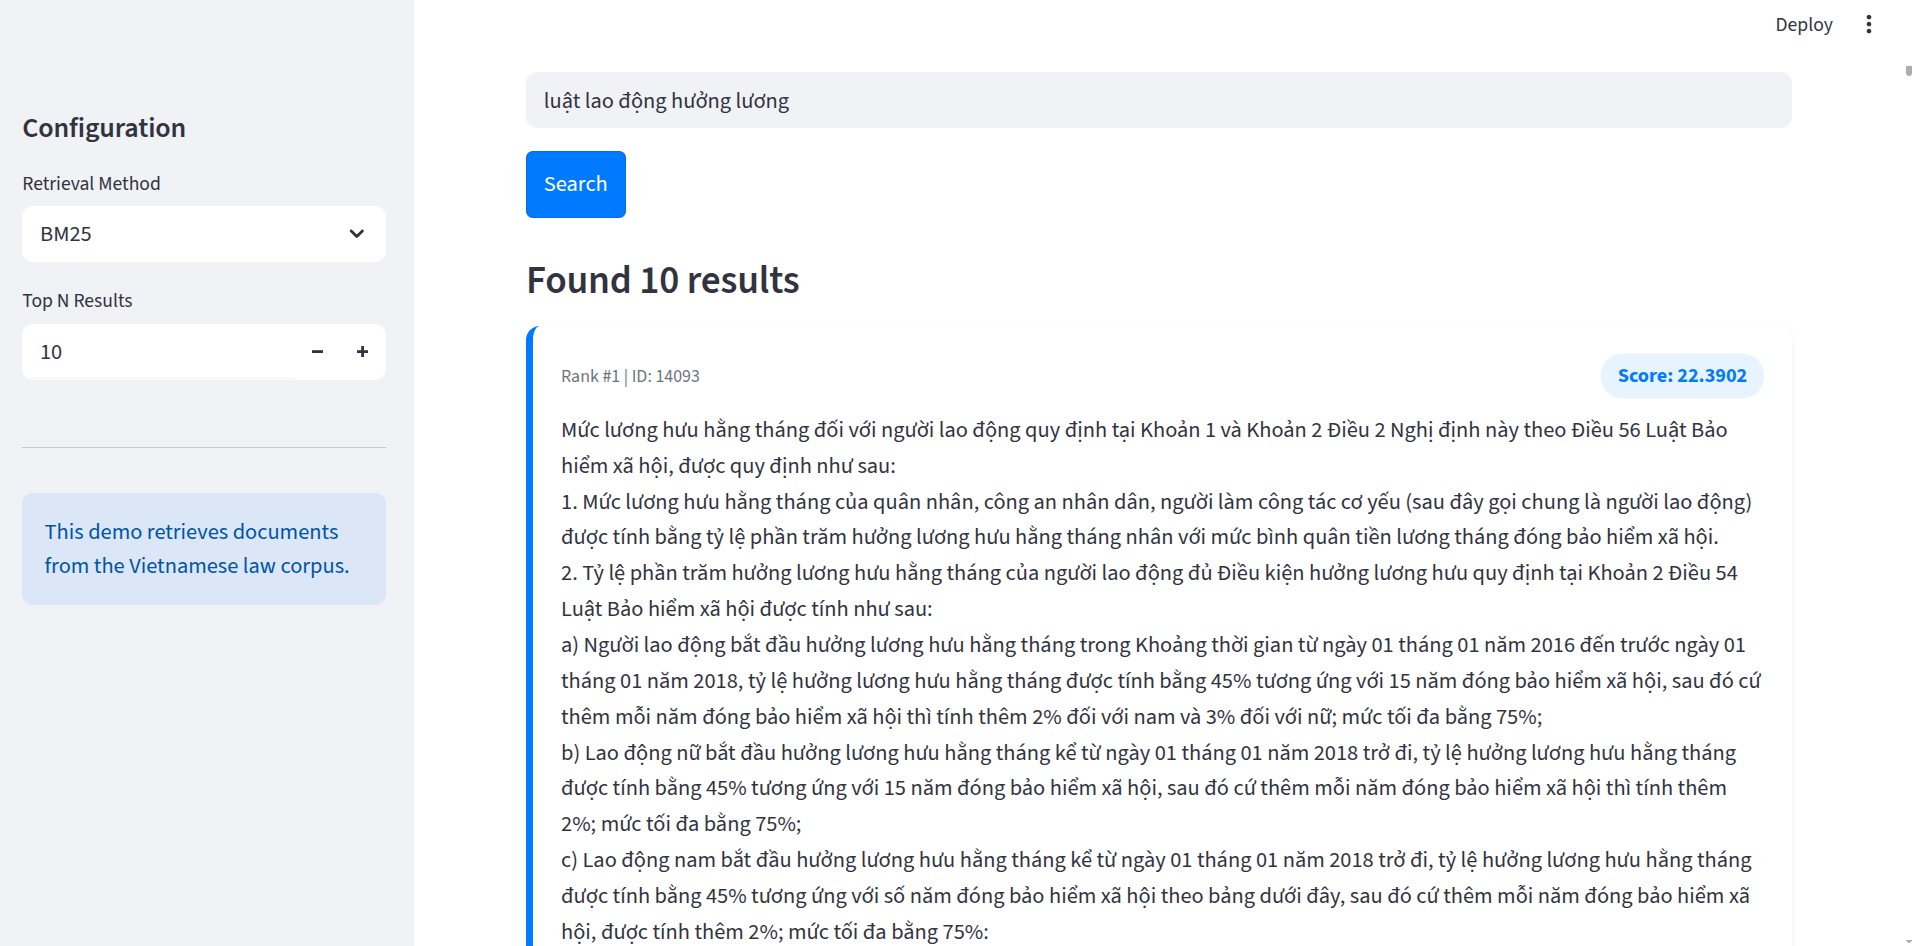
\includegraphics[height=0.8\textheight]{pic/demo-ui.png}
        \label{fig:demo-ui}
\end{figure}
\end{frame}

\begin{frame}{Kết luận}
\begin{itemize}
    \item Đã cài đặt và so sánh thành công 5 phương pháp truy xuất
    \item \textbf{BM25} và \textbf{ES (đã xử lý)} cho kết quả tốt nhất
    \item Tiền xử lý văn bản (tách từ tiếng Việt) quan trọng
    \item Xây dựng giao diện demo hoàn chỉnh với Streamlit
\end{itemize}
\end{frame}

\begin{frame}
\begin{center}
    Cảm ơn thầy đã lắng nghe!
\end{center}
\end{frame}

\begin{frame}[t, allowframebreaks]
\frametitle{Tài liệu tham khảo}
\bibliography{sample}
\end{frame}

\end{document}